
\documentclass[12pt]{article}
\usepackage{amsmath, amssymb, graphicx, geometry, booktabs}
\geometry{margin=1in}
\usepackage{hyperref}
\hypersetup{colorlinks=true, linkcolor=blue, urlcolor=blue}

\title{\textbf{Taylor-Maccoll Supersonic Cone Flow Simulation}}
\author{Dron Das Purkayastha}
\date{}

\begin{document}
\maketitle

\section*{Objective}
The purpose of this project is to numerically solve the Taylor-Maccoll equation for compressible supersonic flow over a sharp cone using MATLAB. The project performs a grid convergence study, exports flow variable data to CSV, and visualizes the solution to understand the behavior of flow variables across a conical shock.

\section*{Governing Equations}
The Taylor-Maccoll equation models the axisymmetric flow between an oblique shock and the surface of a cone:
\[
\frac{dV_r}{d\psi} = V_\psi, \quad
\frac{dV_\psi}{d\psi} = -\left( \frac{V_r^2 - V_\psi^2}{V_r} + \frac{\gamma - 1}{2}(V_r^2 + V_\psi^2 - 1)\frac{V_\psi}{V_r} \right)
\]
The initial values for \(V_r\) and \(V_\psi\) are obtained from the post-shock flow using oblique shock relations. Integration is carried out using the 4th-order Runge-Kutta method.

\section*{Methodology}
\begin{itemize}
    \item Calculate post-shock Mach number using oblique shock theory.
    \item Integrate the Taylor-Maccoll ODEs starting from the shock angle.
    \item Compute Mach number, pressure, temperature, and density using isentropic relations.
    \item Perform the simulation for different angular step sizes (\(0.1^\circ, 0.2^\circ, 0.4^\circ\)) for grid convergence analysis.
    \item Export the flow field results into a CSV file.
    \item Generate plots using MATLAB to visualize key variables vs. flow angle \(\psi\).
\end{itemize}

\section*{Flow Variables}
The solver computes:
\begin{itemize}
    \item Radial velocity component \(V_r\)
    \item Angular velocity component \(V_\psi\)
    \item Mach number \(M\)
    \item Pressure ratio \(\frac{p}{p_1}\)
    \item Temperature ratio \(\frac{T}{T_1}\)
    \item Density ratio \(\frac{\rho}{\rho_1}\)
\end{itemize}

\section*{Results Overview}
The code outputs a CSV file `flow_data_dpsi_0_2.csv`, which contains 226 data points. Each row corresponds to a discrete angular step from the shock toward the cone surface. This data was plotted to provide deeper insights into how flow variables evolve along the streamline.

\section*{Visualization of Output}
\begin{figure}[h!]
\centering
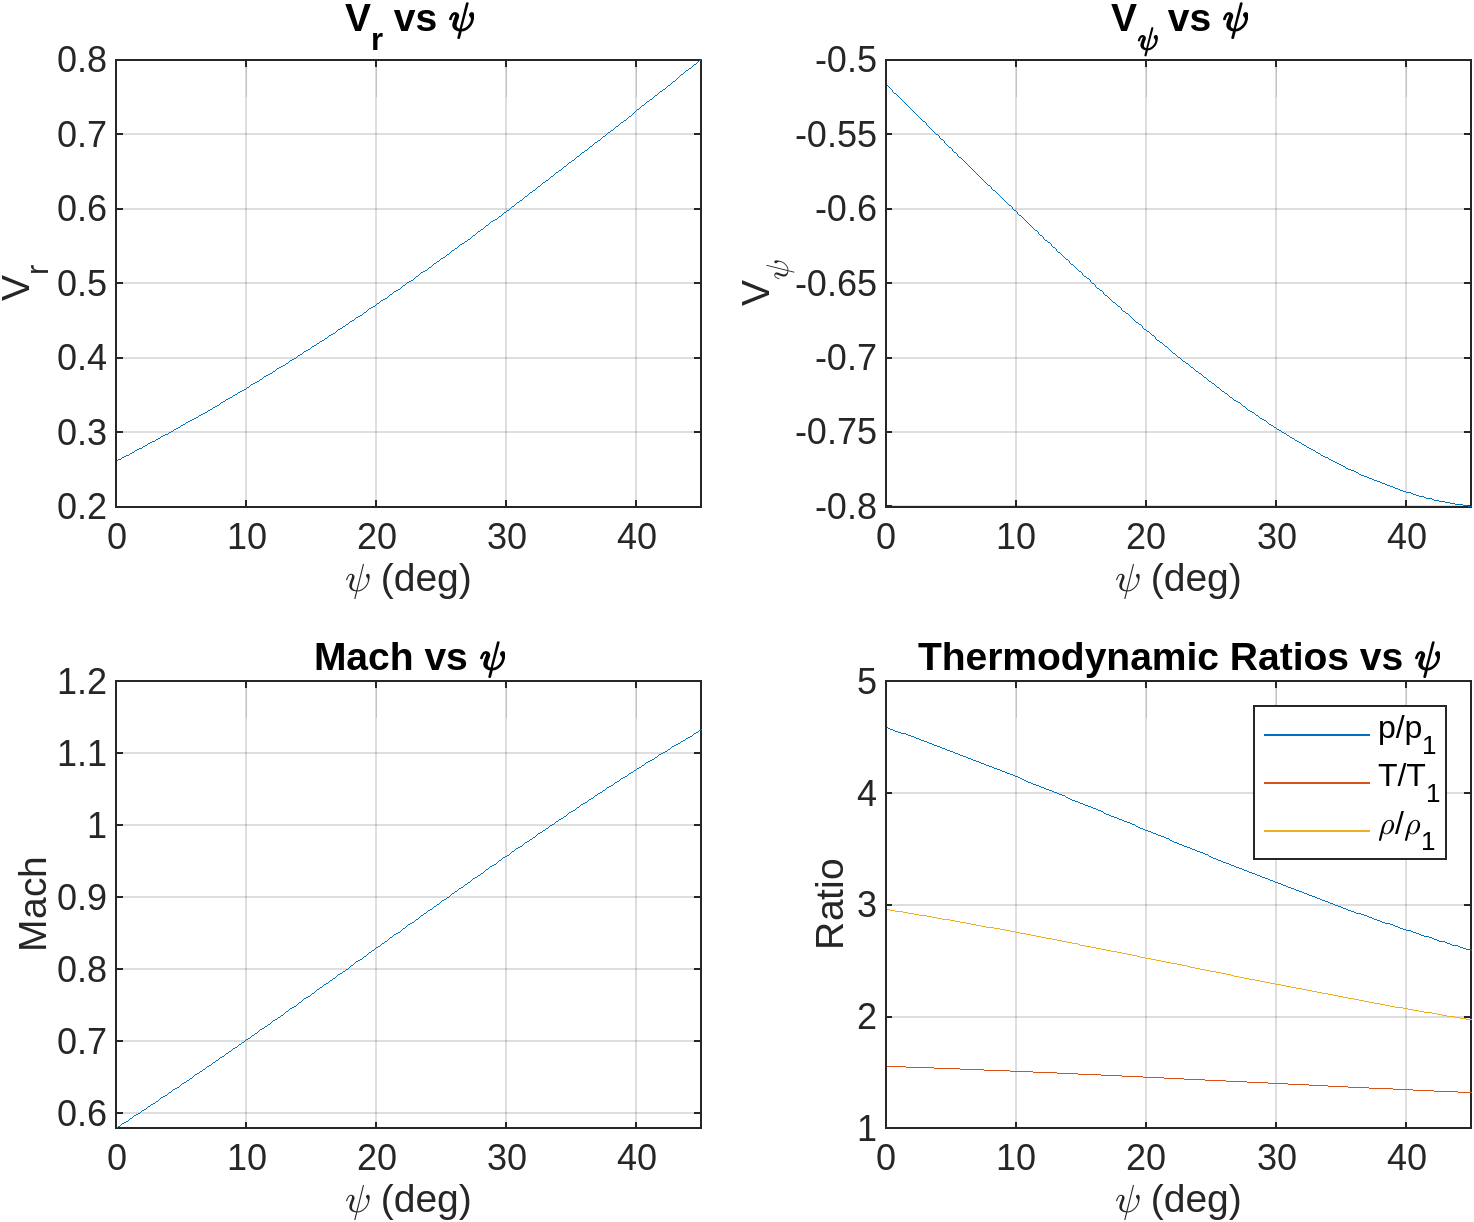
\includegraphics[width=0.9\textwidth]{../plots/flow_distribution_plots.png}
\caption{Visualization of Mach number, pressure, temperature, and velocity components vs. angle \(\psi\)}
\end{figure}

\section*{Inferences}
\begin{itemize}
    \item The Mach number decreases from the shock to the cone due to compression.
    \item Static pressure, temperature, and density increase gradually toward the cone surface.
    \item Grid convergence is confirmed with little variation across step sizes.
    \item The final cone surface values match theoretical expectations.
\end{itemize}

\section*{Conclusion}
The Taylor-Maccoll solver implemented in MATLAB accurately models supersonic flow over a cone. With clean visual output, convergence checks, and physical trends confirmed, this tool serves as a solid reference for supersonic flow analysis in both academic and applied settings.

\end{document}
